\documentclass[../../main]{subfiles}

\begin{document}
\chapter{準備と前提知識}
\label{chapter:preliminary}

\begin{lead}
  \cref{chapter:preliminary}では,素朴集合論・線型代数学・微分積分学で有名な事実を,本書で必要となるものに限って概観する.
\end{lead}

\section{行列とベクトル空間}

\subsection{ベクトル空間}
以下,集合\(\numset{K}\)は実数の全体集合\(\numset{R}\)か,複素数の全体集合\(\numset{C}\)であるとする.
\(\numset{K}\)上のベクトル空間とは次のように定義される,加法とスカラー乗法が備わった集合のことである.

\begin{definition}{ベクトル空間}{vector_space}\index{べくとるくうかん@ベクトル空間}
  \(V\)を空でない集合とする.また,任意の\(\vect{x},\vect{y}\in V\),\(s\in\numset{K}\)について,
  和\(\vect{x}+\vect{y}\in V\)とスカラー倍\(s\vect{x}\in V\)が定義されているとする.
  任意の\(\vect{x},\vect{y},\vect{z}\in V\),\(s,t\in\numset{K}\)に対する以下の条件を満たすとき,
  \(V\)は\(\numset{K}\)上の\termdef{ベクトル空間}(vector space)であるという.

  \begin{enumerate}
    \item \((\vect{x}+\vect{y})+\vect{z}=\vect{x}+(\vect{y}+\vect{z})\)
    \item \(\vect{x}+\vect{y}=\vect{y}+\vect{x}\)
    \item ある\(\zvec\in V\)が存在し,任意の\(\vect{v}\in V\)に対して\(\vect{v}+\zvec=\vect{v}\)を満たす
    \item 各\(\vect{v}\in V\)に対し,ある\(\vect{w}\in V\)が一意に存在して\(\vect{v}+\vect{w}=\zvec\)を満たす
    \item \((s+t)\vect{x}=s\vect{x}+t\vect{x}\)
    \item \(s(\vect{x}+\vect{y})=s\vect{x}+s\vect{y}\)
    \item \((st)\vect{x}=s(t\vect{x})\)
    \item \(1\vect{x}=\vect{x}\)
  \end{enumerate}
\end{definition}

しばしば\(V\)の元をベクトル,\(\numset{K}\)の元をスカラーと呼ぶ.
また,\cref{definition:vector_space}の\(\zvec\)を\termdef{零ベクトル}\index{ぜろべくとる@零ベクトル}(zero vector),\(\vect{w}\)を\(\vect{v}\)の\termdef{加法逆元}\index{かほうぎゃくげん@加法逆元}(additive inverse)という.
通常,\(\vect{v}\)の加法逆元は\(-\vect{v}\)と表される.

\begin{note}
  \cref{definition:vector_space}はごてごてしているように見えるが,
  それは和とスカラー倍について,\(\numset{K}^n\)と同様に計算できるよう,ルールをつけ加えていった結果といえる.
\end{note}

ついで,ベクトル空間にかかわる概念を2つ定義する.これらの関係については,すぐ後で説明する.

\begin{definition}{線型結合}{linear_combination}\index{せんけいけつごう@線型結合}
  \(V\)を\(\numset{K}\)上のベクトル空間,\(\vect{v}_1,\dots,\vect{v}_n\)を\(V\)の元とする.
  \(c_1\vect{v}_1+\dots+c_n\vect{v}_n\)(\(c_1,\dots,c_n\in\numset{K}\))という形をした\(V\)の元を,
  \(\vect{v}_1,\dots,\vect{v}_n\)の\termdef{線型結合}(linear combination)という.
\end{definition}

\begin{definition}{部分空間}{subspace}\index{べくとるくうかん@ベクトル空間!ぶぶん@部分—|see{部分空間}}\index{ぶぶんくうかん@部分空間}
  \(V\)を\(\numset{K}\)上のベクトル空間,\(W\)を\(V\)の空でない部分集合とする.
  \(W\)が\(V\)の加法とスカラー乗法について\cref{definition:vector_space}の条件をすべて満たすとき,
  \(W\)は\(V\)の\termdef{部分ベクトル空間}(vector subspace),あるいは単に\termdef{部分空間}(subspace)であるという.    
\end{definition}

ある部分集合\(W\subset V\)が\(V\)の部分空間かどうか調べるには,\cref{proposition:subspace_iff}を使うとよい.

\begin{proposition}{}{subspace_iff}
  \(V\)を\(\numset{K}\)上のベクトル空間,\(W\)を\(V\)の空でない部分集合とする.このとき,次の命題は同値である.
  \begin{enumerate}
    \item \(W\)は\(V\)の部分空間である
    \item 任意の\(s\in\numset{K}\),\(\vect{w}_1,\vect{w}_2\in W\)に対して\(s\vect{w}_1,\vect{w}_1+\vect{w}_2\in W\)である
  \end{enumerate}
\end{proposition}

\begin{example}
  \(V\)が\(\numset{K}\)上のベクトル空間なら,\(V\)自身と\(\Set{\zvec}\)は\(V\)の部分空間である.
\end{example}

\begin{example}
  集合\(\numset{K}^n=\Set{\trps{\inlinevec{s_1 & \cdots & s_n}}\given s_1,\dots,s_n\in\numset{K}}\)は,
  通常の加法とスカラー乗法によって,\(\numset{K}\)上のベクトル空間になる.
\end{example}

また,2つの部分空間\(W_1,W_2\subset V\)があれば,それらを含むより大きな部分空間を作れる.

\begin{definition}{部分空間の和}{sum_of_subspace}\index{ぶぶんくうかん@部分空間!のわ@—の和}\index{\(W_1+W_2\)}
  \(V\)を\(\numset{K}\)上のベクトル空間,\(W_1,W_2\subset V\)を部分空間とする.
  このとき,集合\(W=\Set{\vect{w}_1+\vect{w}_2\given\text{\(\vect{w}_1\in W_1\),\(\vect{w}_2\in W_2\)}}\)は\(V\)の部分空間になる.
  \(W\)を\(W_1\)と\(W_2\)の\termdef{和}(sum)といい,\(W_1+W_2\)と表記する.
\end{definition}

特に\(W_1\cap W_2=\Set{\zvec}\)であるとき,\(W_1+W_2\)を\(W_1\)と\(W_2\)の\termdef{直和}\index{ぶぶんくうかん@部分空間!のちょくわ@—の直和}(direct sum)という.
直和であることを強調したいときは,和\(W_1+W_2\)を\(W_1\oplus W_2\)\index{\(W_1\oplus W_2\)}とも書く.

\subsection{基底}
任意のベクトル\(\vect{x}=\trps{\inlinevec{x_1 & \cdots & x_n}}\in\numset{K}^n\)は,第\(i\)成分が\(1\),他の成分が\(0\)のベクトル\(\vect{e}_i\)を用いて
\(\vect{x}=x_1\vect{e}_1+\dots+x_n\vect{e}_n\)と表せる.
すなわち,集合\(\basis{S}_n=\Set{\vect{e}_1,\dots,\vect{e}_n}\)は「\(\numset{K}^n\)のすべての元を\(\basis{S}_n\)の元の線型結合で書ける」という性質を持つ.

一般に,ベクトル空間\(V\)の部分集合\(S\)に対して,\(S\)の元の線型結合で書けるベクトルの全体集合を\(S\)が\termdef{生成する部分空間}\index{ぶぶんくうかん@部分空間!せいせいする@生成する—}(generated subspace)といい,
\(\spannedby S\)\index{\(\spannedby S\)}と表記する.この記法を使えば,先述した\(\basis{S}_n\)が持つ性質を「\(\spannedby\basis{S}_n=\numset{K}^n\)が成り立つ」と言い換えられる.

\(\spannedby S=\numset{K}^n\)を満たす集合\(S\subset\numset{K}^n\)は,\(\basis{S}_n\)以外にも無数にある.
たとえば\(\numset{K}^n=\numset{R}^2\)のとき,集合\(T=\Set{\trps{\inlinevec{1 & 1}},\trps{\inlinevec{2 & -1}},\trps{\inlinevec{-1 & 0}}}\)が生成する部分空間は
\(\numset{R}^2\)である.しかし,\(\basis{S}_2=\Set{\trps{\inlinevec{1 & 0}},\trps{\inlinevec{0 & 1}}}\)の元の線型結合で\(\numset{R}^2\)の元を表す方法はただ1通りであるのに対して,\(T\)はこの性質を持たない(\cref{figure:linear_comb}).

\begin{figure}[htbp]
  \centering
  \begin{minipage}{\linewidth/2}
    \centering
    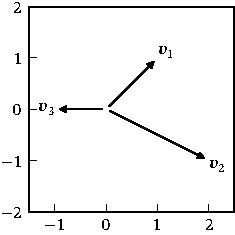
\includegraphics{linear_comb1.pdf}
  \end{minipage}%
  \begin{minipage}{\linewidth/2}
    \centering
    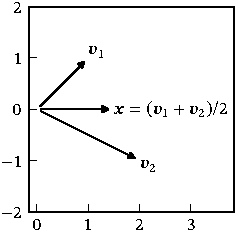
\includegraphics{linear_comb2.pdf}    
  \end{minipage}
  \caption{\(\vect{v}_1,\vect{v}_2,\vect{v}_3\in T\)の線型結合で\(\vect{x}=\trps{[\begin{matrix}3/2 & 0\end{matrix}]}\)を表した様子.明らかに\(\vect{x}=(-3/2)\vect{v}_3\)である一方,\(\vect{x}=(\vect{v}_1+\vect{v}_2)/2=(1/2)\vect{v}_1+(1/2)\vect{v}_2\)も成り立つ.}
  \label{figure:linear_comb}
\end{figure}

\(S\)の元の線型結合で\(\spannedby S\)の元を一意に表せるとき,任意の\(a_i,b_i\in\numset{K}\),\(\vect{v}_i\in S\)について
\[
  \sum_{i=1}^ka_i\vect{v}_i = \sum_{i=1}^kb_i\vect{v}_i
  \implies \begin{bmatrix}a_1 & \cdots & a_k\end{bmatrix} = \begin{bmatrix}b_1 & \cdots & b_k\end{bmatrix} 
\]
が成立する.\(b_1=\dots=b_k=0\)とすると
\begin{equation}
  \label{equation:independence}
  a_1\vect{v}_1+\dots+a_k\vect{v}_k = \zvec
  \implies a_1 = \dots = a_k = 0
\end{equation}
が得られる.

任意の\(a_1,\dots,a_k\in\numset{K}\)に対して\cref{equation:independence}が成立するとき,
\(\vect{v}_1,\dots,\vect{v}_k\)は\termdef{線型独立}であるという.特に,\(V=\spannedby S\)かつ,\(S\)の元からなる有限個のベクトルの組が常に線型独立であるとき,\(S\)は\(V\)の\termdef{基底}であるという.
以上を\cref{definition:independence,definition:basis}にまとめておく.

\begin{definition}{生成系・線型独立・線型従属}{independence}
  \(V\)を\(\numset{K}\)上のベクトル空間,\(S\)を\(V\)の部分集合とする.また,\(\vect{v}_1,\dots,\vect{v}_k\)を\(V\)の元とする.
  \begin{enumerate}
    \item \(V=\spannedby S\)であるとき,\(S\)を\(V\)の\termdef{生成系}(generating set)という
    \item \(\sum_{i=1}^kc_i\vect{v}_i=\zvec\)を満たす\(c_1,\dots,c_k\in\numset{K}\)の組が\(c_1=\dots=c_k=0\)しかないとき,\(\vect{v}_1,\dots,\vect{v}_k\)は\termdef{線型独立}\index{せんけいどくりつ@線型独立}(linearly independent)であるという
    \item \(\vect{v}_1,\dots,\vect{v}_k\)が線型独立でないとき,\(\vect{v}_1,\dots,\vect{v}_k\)は\termdef{線型従属}\index{せんけいじゅうぞく@線型従属}(linearly dependent)であるという
  \end{enumerate}
\end{definition}

\begin{definition}{基底}{basis}
  \(V\)を\(\numset{K}\)上のベクトル空間,\(\basis{B}\)を\(V\)の部分集合とする.
  \(\basis{B}\)が\(V\)の生成系かつ,\(\basis{B}\)に属する有限個のベクトル\(\vect{v}_1,\dots,\vect{v}_k\)が常に線型独立であるとき,\(\basis{B}\)は\(V\)の\termdef{基底}\index{きてい@基底}(basis)であるという.
\end{definition}

\begin{example}[標準基底]
  \(\basis{S}_n\)は\(\numset{K}^n\)の基底である.\(\basis{S}_n\)を\(\numset{K}^n\)の\termdef{標準基底}\index{ひょうじゅんきてい@標準基底}(standard basis)という.
\end{example}

さきほどの議論によれば,\(S\)の元の線型結合で\(\spannedby S\)の元を一意に表せるとき,任意の\(a_1,\dots,a_k\in\numset{K}\)について\cref{equation:independence}が成立する.
すなわち,\(S\)は\(\spannedby S\)の基底である.実はこの逆も示せるので,次の命題が成立する.

\begin{proposition}{}{span_and_uniqueness}
  \(V\)を\(\numset{K}\)上のベクトル空間,\(S\)を\(V\)の部分集合とする.このとき,次の命題は同値である.
  \begin{enumerate}
    \item \(S\)の元の線型結合で\(\spannedby S\)の元を一意に表せる
    \item \(S\)は\(\spannedby S\)の基底である
  \end{enumerate}
\end{proposition}

\(V\)の基底で有限集合のものがあるとき,\(V\)は\termdef{有限次元}\index{ゆうげんじげん@有限次元}(finite-dimensional)であるという.
\(V\)が有限次元なら,\(V\)の基底はすべて有限集合で,その元の個数は等しい.
すなわち,元の個数\(\sizeof{\basis{B}}\)は基底\(\basis{B}\)のとりかたによらず定まる.
\(\sizeof{\basis{B}}\)を\(V\)の\termdef{次元}\index{じげん@次元}(dimension)といい,\(\dim V\)\index{\(\dim V\)}と表記する
\footnote{\(V\)が有限次元でないときも基底は存在する(証明は文献\cite{yukie2019}).}.

基底に関連して,次の命題が成り立つ.

\begin{proposition}{基底の延長}{basis_extension}
  \(V\)を\(\numset{K}\)上の\(n\)次元ベクトル空間とする.\(k<n\)個のベクトル\(\vect{v}_1,\dots,\vect{v}_k\in V\)が線型独立なら,
  集合\(\Set{\vect{v}_1,\dots,\vect{v}_k,\vect{v}_{k+1},\dots,\vect{v}_n}\)が\(V\)の基底になる\(\vect{v}_{k+1},\dots,\vect{v}_n\in V\)が存在する.
\end{proposition}

\subsection{内積}
\(\numset{R}^3\)において,ベクトルの長さとなす角はドット積\((x_1,x_2,x_3)\cdot(y_1,y_2,y_3)=\sum_{i=1}^3x_iy_i\)から計算できた.
\cref{definition:inner_product}は,こうした幾何的な考察を,より多くのベクトル空間へと適用可能にする.

\begin{definition}{内積}{inner_product}\index{ないせき@内積}\index{\(\innerp{\holder}{\holder}\)}
  \(V\)を\(\numset{K}\)上のベクトル空間とする.\(\innerp{\holder}{\holder}\)が\(V\)の\termdef{内積}(inner product)であるとは,
  任意の\(\lambda\in\numset{K}\),\(\vect{x},\vect{y},\vect{z}\in V\)に対し,\(\innerp{\holder}{\holder}\)が以下の条件を満たすことをいう.
  \begin{enumerate}
    \item \(\innerp{\vect{x}}{\vect{y}}=\conj{\innerp{\vect{y}}{\vect{x}}}\)
    \item \(\innerp{\lambda\vect{x}+\vect{y}}{\vect{z}}=\lambda\innerp{\vect{x}}{\vect{z}}+\innerp{\vect{y}}{\vect{z}}\)
    \item \(\innerp{\vect{x}}{\vect{x}}\geq 0\),\([\innerp{\vect{x}}{\vect{x}}=0\iff\vect{x}=\zvec]\)
  \end{enumerate}
\end{definition}

内積が備わっているベクトル空間のことを\termdef{内積空間}\index{ないせきくうかん@内積空間}(inner product space)という.
また,\(\innerp{\vect{v}}{\vect{w}}=0\)であるとき,ベクトル\(\vect{v}\)と\(\vect{w}\)は\termdef{直交}\index{ちょっこう@直交}するという.

\begin{note}
  定義により,\(\zvec\)は任意のベクトルと直交する.この事実は直感にそぐわないかもしれないが,\(\zvec\)だけを特別扱いするとかえって面倒である.
\end{note}

\begin{example}[標準内積]
  \(\innerp{\vect{v}_1}{\vect{v}_2}=\trps{\vect{v}_1}\conj{\vect{v}_2}\)(\(\vect{v}_1,\vect{v}_2\in\numset{K}^n\))とすると,
  \(\innerp{\holder}{\holder}\)は\(\numset{K}^n\)の内積になる.\(\innerp{\holder}{\holder}\)を\(\numset{K}^n\)の\termdef{標準内積}\index{ひょうじゅんないせき@標準内積}という.
\end{example}

\cref{definition:onb}は,本書の中核をなす重要な概念である.

\begin{definition}{正規直交系,正規直交基底}{onb}\index{せいきちょっこうけい@正規直交系}\index{せいきちょっこうきてい@正規直交基底}
  \(V\)を内積空間とする.集合\(\basis{B}\subset V\)が\termdef{正規直交系}(orthonormal system; ONS)であるとは,任意の\(\vect{e}_1,\vect{e}_2\in\basis{B}\)が条件
  \[
    \innerp{\vect{e}_1}{\vect{e}_2} = \begin{cases}1 & (\vect{e}_1=\vect{e}_2),\\ 0 & (\vect{e}_1\neq\vect{e}_2)\end{cases}
  \]
  を満たすことをいう.また,\(\basis{B}\)が\(V\)の基底であるとき,\(\basis{B}\)は\termdef{正規直交基底}(orthonormal basis; ONB)であるという.
\end{definition}

\(\basis{B}\)が正規直交系なら,有限個の\(\vect{e}_1,\dots,\vect{e}_k\in\basis{B}\)は常に線型独立である.
よって,\(\basis{B}\)が基底であることを見るには,\(V=\spannedby\basis{B}\)だけ確認すればよい.

また,内積空間に属する線型独立なベクトルの組があれば,それらから正規直交系を作れる.

\begin{proposition}{}{gram_schmidt}
  \(V\)を内積空間とする.\(\vect{v}_1,\dots,\vect{v}_k\in V\)が線型独立なら,式
  \[
    \vect{u}_1 = \vect{v}_1,
    \quad\vect{u}_i = \vect{v}_i-\sum_{j=1}^{i-1}\frac{\innerp{\vect{u}_j}{\vect{v}_j}}{\innerp{\vect{u}_j}{\vect{u}_j}}\vect{u}_j\quad(i=2,\dots,k)
  \]
  でベクトル\(\vect{u}_1,\dots,\vect{u}_k\)を定義すると,集合\(\narrowbaselines\Set{\vect{u}_i/\sqrt{\innerp{\vect{u}_i}{\vect{u}_i}}\given i=1,\dots,k}\)は正規直交系になる.
\end{proposition}

正規直交系を作る\cref{proposition:gram_schmidt}の方法を\termdef{グラム・シュミットの直交化法}\index{ぐらむしゅみっとのちょっこうかほう@グラム・シュミットの直交化法}(Gram–Schmidt orthogonalization)という.
\cref{proposition:gram_schmidt}から,有限次元の内積空間は常に正規直交基底を持つ.

\subsection{線型写像と表現行列}
\(V\)は有限次元であるとする.\cref{proposition:span_and_uniqueness}によれば,\(V\)の基底\(\basis{B}=\Set{\vect{v}_1,\dots,\vect{v}_m}\)(\(m=\dim V\))をとることで,
任意の\(\vect{x}\in V\)を
\begin{equation}
  \label{equation:basis_comb}
  \vect{x} = c_1\vect{v}_1+\dots+c_m\vect{v}_m\quad(c_1,\dots,c_m\in\numset{K})
\end{equation}
の形で一意に表せる.言い換えると,\(V\)の各元\(\vect{x}\)に\cref{equation:basis_comb}の\(\trps{\inlinevec{c_1 & \cdots & c_m}}\)を割り当てる写像\(\phi\colon V\to\numset{K}^m\)を定義でき,
それは単射\footnote{写像\(f\)の定義域に属する任意の\(x,y\)について,命題「\(f(x)=f(y)\implies x=y\)」が成立するとき,\(f\)は\termdef{単射}(injection)であるという.}\index{たんしゃ@単射}である.
この写像\(\phi\)は,次に定義する「線型写像」の1例である.

\begin{definition}{線型写像}{linear_mapping}\index{せんけいしゃぞう@線型写像}
  \(V\)と\(W\)を\(\numset{K}\)上のベクトル空間とする.写像\(f\colon V\to W\)が以下の条件を満たすとき,\(f\)は\termdef{線型写像}(linear mapping)であるという.
  \begin{enumerate}
    \item 任意の\(\vect{x},\vect{y}\in V\)に対して\(f(\vect{x}+\vect{y})=f(\vect{x})+f(\vect{y})\)
    \item 任意の\(\vect{x}\in V\),\(c\in\numset{K}\)に対して\(f(c\vect{x})=cf(\vect{x})\)
  \end{enumerate}
\end{definition}

\(W\)を\(\numset{K}\)上の有限次元ベクトル空間とする.\(W\)の基底\(\basis{B}'=\Set{\vect{w}_1,\dots,\vect{w}_n}\)(\(n=\dim W\))をとると,
\(\phi\)と同様
\[
  \vect{y} = d_1\vect{w}_1+\dots+d_n\vect{w}_n
  \iff\psi(\vect{y}) = \trps{\begin{bmatrix}d_1 & \cdots & d_n\end{bmatrix}}
\]
を満たす線型写像\(\psi\colon W\to\numset{K}^n\)が定義できる.

\(\phi\)と\(\psi\)を利用すると,\(V\)から\(W\)への任意の線型写像\(f\)を,対応する行列によって表現できる.
\(\vect{x}\in V\)を任意にとる.\(\phi(\vect{x})=\trps{\inlinevec{c_1 & \cdots & c_m}}\)とおくと
\[
  f(\vect{x}) = f\pqty*{\sum_{i=1}^mc_i\vect{v}_i} = \sum_{i=1}^mc_if(\vect{v}_i)
\]
であるから
\[
  \psi(f(\vect{x})) = \sum_{i=1}^mc_i\psi(f(\vect{v}_i))
  = \begin{bmatrix}\psi(f(\vect{v}_1)) & \cdots & \psi(f(\vect{v}_m))\end{bmatrix}\begin{bmatrix}c_1 \\ \vdots \\ c_m\end{bmatrix}
\]
となる.よって,\(\mat{A}=\inlinevec{\psi(f(\vect{v}_1)) & \cdots & \psi(f(\vect{v}_m))}\)とおくと,式
\begin{equation}
  \label{equation:representation_matrix}
  \psi(f(\vect{x})) = T(\phi(\vect{x}))\quad(T(\vect{x})=\mat{A}\vect{x})
\end{equation}
が成り立つ.

\begin{wrapfigure}{o}{0pt}
  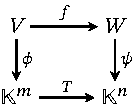
\includegraphics{commute.pdf}
\end{wrapfigure}

ここまでの議論をまとめると,次のようになる.
\(V\)の基底\(\basis{B}\)と,\(W\)の基底\(\basis{B}'\)をとるごとに,
\(n\times m\)行列\(\mat{A}=\inlinevec{\psi(f(\vect{v}_1)) & \cdots & \psi(f(\vect{v}_m))}\)
を定義でき,\(\mat{A}\)は\cref{equation:representation_matrix}を満たす.
この\(\mat{A}\)を,基底\(\basis{B}\)と\(\basis{B}'\)に関する\(f\)の\termdef{表現行列}\index{ひょうげんぎょうれつ@表現行列}(representation matrix)という.

なお,\(\basis{B}\)の元を並べる順序に応じて,\cref{equation:basis_comb}の\(c_1,\dots,c_n\)の順序も変化するので,
\(\phi\)は\(\basis{B}\)に対して一意ではない.\(\phi\)は\(\basis{B}\)の元を並べる順序を決めて初めて定まる.
本書では,\(\basis{B}=\Set{\vect{v}_1,\dots,\vect{v}_n}\)のような書き方をした場合,
\(\basis{B}\)の元を\(\vect{v}_i\)の添え字\(i\)について昇順に並べると決めておく.

\begin{example}[形式的な微分]
  \(n\)次以下の1変数多項式全体\(V_n=\Set{c_0+c_1x+\dots+c_nx^n\given c_0,\dots,c_n\in\numset{R}}\)は,\(\numset{R}\)上の\(n+1\)次元ベクトル空間である.
  また,写像\(D\colon V_3\to V_2\)を
  \[
    D(c_0+c_1x+c_2x^2) = c_1+2c_2x\quad(c_0,c_1,c_2\in\numset{R})
  \]
  で定義すると,これは線型写像になる.\(V_n\)の基底として\(\basis{B}_n=\Set{1,x,\dots,x^n}\)をとったとき,
  基底\(\basis{B}_3\)と\(\basis{B}_2\)に関する\(D\)の表現行列は\(\begin{bsmallmatrix}0 & 1 & 0 \\ 0 & 0 & 2\end{bsmallmatrix}\)である.
\end{example}

\subsection{核と像}
線型写像に付随して,重要なベクトル空間が2つ定まる.

\begin{definition}{核,像}{nul_img}\index{かく@核}\index{ぞう@像}\index{\(\nul f\)}\index{\(\img f\)}
  \(f\colon V\to W\)を線型写像とする.
  \begin{enumerate}
    \item 集合\(\Set{\vect{v}\in V\given f(\vect{v})=\zvec}\)を\(f\)の\termdef{核}(kernel)といい,\(\nul f\)と表す
    \item 集合\(\Set{f(\vect{v})\given\vect{v}\in V}\)を\(f\)の\termdef{像}(image)といい,\(\img f\)と表す
  \end{enumerate}
\end{definition}

一般に,\(\nul f\)と\(\img f\)はそれぞれ\(V\)と\(W\)の部分空間になる.\(\nul f\)について,次の命題が成立する.

\begin{proposition}{}{nul_and_uniqueness}
  \(f\colon V\to W\)を線型写像とする.このとき,\(f\)が単射であることと,\(\nul f=\Set{\zvec}\)が成立することは同値である.
\end{proposition}

\begin{proof}
  \(f(\zvec)=f(\zvec+\zvec)=f(\zvec)+f(\zvec)\)なので,\(f(\zvec)=\zvec\)である.
  よって,\(f\)が単射なら\(f(\vect{v})=\zvec\iff\vect{v}=\zvec\)だから,\(\nul f=\Set{\zvec}\)である.

  また,\(\vect{v}_1,\vect{v}_2\in V\)が\(f(\vect{v}_1)=f(\vect{v}_2)\)を満たせば
  \(f(\vect{v}_1-\vect{v}_2)=f(\vect{v}_1)-f(\vect{v}_2)=\zvec\)である.
  よって,\(\nul f=\Set{\zvec}\)なら\(\vect{v}_1-\vect{v}_2=\zvec\),\(\vect{v}_1=\vect{v}_2\)である.
  すなわち,\(\nul f=\Set{\zvec}\)なら\(f\)は単射である.
\end{proof}

\subsection{固有値と固有空間}
対角化に向けて,固有値に関連する事項を整理する.

\begin{definition}{固有値,固有ベクトル}{eigenvalue}\index{こゆうち@固有値}\index{こゆうべくとる@固有ベクトル}
  \(\mat{A}\)を\(n\)次正方行列とする.
  複素数\(\lambda\)と\(\zvec\)でないベクトル\(\vect{x}\in\numset{C}^n\)が式\(\mat{A}\vect{x}=\lambda\vect{x}\)を満たすとき,
  \(\lambda\)を\(\mat{A}\)の\termdef{固有値}(eigenvalue)という.
  また,\(\vect{x}\)を\(\mat{A}\)の(固有値\(\lambda\)に属する)\termdef{固有ベクトル}(eigenvector)という.
\end{definition}

\begin{example}
  \(\vect{x}_1=\trps{\inlinevec{1+\iuni & 2}}\),\(\vect{x}_2=\trps{\inlinevec{1-\iuni & 2}}\)は\(\mat{A}=\begin{bsmallmatrix}1 & -1 \\ 2 & -1\end{bsmallmatrix}\)の固有ベクトルである.
  実際\(\mat{A}\vect{x}_1=\iuni\vect{x}_1\),\(\mat{A}\vect{x}_2=-\iuni\vect{x}_2\)である.
\end{example}

\cref{definition:eigenvalue}を満たす\(\lambda\)を見つけるには,次の\cref{proposition:characteristic_polynomial}を利用するとよい.

\begin{proposition}{}{characteristic_polynomial}
  \(\lambda\)が正方行列\(\mat{A}\)の固有値であることと,\(\det(\lambda\imat-\mat{A})=0\)であることは同値である.
  ただし,\(\det\mat{A}\)は\(\mat{A}\)の行列式\index{ぎょうれつしき@行列式}である.
\end{proposition}

\(n\)次多項式\(P(\lambda)=\det(\lambda\imat-\mat{A})\)を\(\mat{A}\)の\termdef{固有多項式}\index{こゆうたこうしき@固有多項式}(characteristic polynomial)という.
\cref{proposition:characteristic_polynomial}から,集合\(\Set{\lambda\in\numset{C}\given P(\lambda)=0}\)は\(\mat{A}\)の固有値の全体集合である.

\begin{corollary}{}{eigen_size}
  任意の\(n\)次正方行列\(\mat{A}\)は,相異なる固有値を少なくとも1個,多くとも\(n\)個もつ.
\end{corollary}

\begin{proof}
  \(\det(\lambda\imat-\mat{A})=0\)は\(\lambda\)に関する\(n\)次方程式なので,解は存在しても\(n\)個以下である.また,代数学の基本定理より解は少なくとも1つ存在する.
\end{proof}

\begin{definition}{固有空間}{eigenspace}\index{こゆうくうかん@固有空間}\index{\(E_\lambda(\mat{A})\)}
  \cref{definition:eigenvalue}の\(\mat{A}\),\(\lambda\)について,集合
  \[
    E_\lambda(\mat{A}) = \Set{\vect{x}\in\numset{C}^n\given\mat{A}\vect{x}=\lambda\vect{x}}
  \]
  は\(\numset{C}^n\)の部分空間になる.部分空間\(E_\lambda(\mat{A})\)を,
  \(\mat{A}\)の(固有値\(\lambda\)に属する)\termdef{固有空間}(eigenspace)という.
\end{definition}

固有空間は次の性質を持つ.

\begin{proposition}{}{eigenspaces_disjointness}
  \(\lambda_1\),\(\lambda_2\)を正方行列\(\mat{A}\)の固有値とする.このとき,次の命題が成立する.
  \begin{enumerate}
    \item \(\vect{x}\in E_{\lambda_1}(\mat{A})\implies\mat{A}\vect{x}\in E_{\lambda_1}(\mat{A})\)
    \item \(\lambda_1\neq\lambda_2\implies E_{\lambda_1}(\mat{A})\cap E_{\lambda_2}(\mat{A})=\Set{\zvec}\)
  \end{enumerate}
\end{proposition}

\begin{proof}
  後半のみ示す.\(\mat{A}\zvec=\lambda_1\zvec=\lambda_2\zvec=\zvec\)なので,\(\zvec\in E_{\lambda_1}(\mat{A})\cap E_{\lambda_2}(\mat{A})\)である.
  また,任意に\(\vect{x}\in E_{\lambda_1}(\mat{A})\cap E_{\lambda_2}(\mat{A})\)をとると,\(\mat{A}\vect{x}=\lambda_1\vect{x}=\lambda_2\vect{x}\)だから\((\lambda_1-\lambda_2)\vect{x}=\zvec\)である.
  \(\lambda_1\neq\lambda_2\)なので\(\vect{x}=\zvec\)である.よって,\(E_{\lambda_1}(\mat{A})\cap E_{\lambda_2}(\mat{A})\)は\(\zvec\)以外に元を持たない.
\end{proof}

\subsection{対角化}
適当な\(n\)次正則行列\(\mat{P}\),対角行列\(\mat{\Lambda}\)の組を見つけて,\(n\times n\)行列\(\mat{A}\)を\(\mat{A}=\mat{P}\mat{\Lambda}\mat{P}^{-1}\)の形で書くことを
\(\mat{A}\)の\termdef{対角化}\index{たいかくか@対角化}(diagonalization)という.
\(\mat{A}\)が対角化可能である必要十分条件は,次の\cref{proposition:diagonalization}で与えられる.

\begin{proposition}{}{diagonalization}
  \(n\)次正方行列\(\mat{A}\)の固有値全体を\(\Set{\lambda_1,\dots,\lambda_k}\)とおく.ただし,\(i\neq j\)ならば\(\lambda_i\neq\lambda_j\)とする.
  このとき,次の命題は同値である.

  \begin{enumerate}
    \item \(\mat{A}\)の固有ベクトルのみからなる\(\numset{K}^n\)の基底が存在する
    \item \(\numset{K}^n=E_{\lambda_1}(\mat{A})\oplus\dots\oplus E_{\lambda_k}(\mat{A})\)が成立する
    \item \(n\)次正則行列\(\mat{P}\),対角行列\(\mat{\Lambda}\)が存在して\(\mat{\Lambda}=\mat{P}^{-1}\mat{A}\mat{P}\)を満たす
  \end{enumerate}
\end{proposition}

\section*{演習問題}
\addcontentsline{toc}{section}{演習問題}

\end{document}
